\documentclass[11pt,a4paper]{report}
\usepackage[hmargin=1.25in,vmargin=1in]{geometry}
\usepackage{amsthm,cite,url,amsmath,amssymb,bm}
\usepackage{algorithm,graphicx,color,mathtools}
\usepackage{physics,enumitem,thmtools}
\usepackage{hyperref,tikz,caption}
\usepackage[english]{babel}
\widowpenalty=4000
\clubpenalty=4000

\title{The Solution of Model Predictive Control: Theory, Computation, and Design \cite{rawlings2017model}}
\author{lixc21}
\date{\today}



\newtheorem*{remark}{Remark}
\theoremstyle{definition}\newtheorem{exercise}{Exercise}[chapter]
\declaretheoremstyle[
  headfont=\color{blue}\normalfont\bfseries,
  bodyfont=\color{blue}\normalfont,
]{colored}
\declaretheorem[
  style=colored,
  name=Answer,
]{answer}



\begin{document}
\maketitle
\tableofcontents
\chapter{Getting Started with Model Predictive Control}
\section{Brief Review}
In this section, we just consider state space linear time invariant system with zero steady state.

\paragraph{Lemma 1.3} (LQR convergence). For $(A,B)$ controllable, the infinite LQR gives a convergent closed-loop system.
\begin{proof}
Because $(A,B)$ is controllable, there exists a sequence of $n$ inputs that transfers the state to zero. When $k>n$, we let $u=0$, then the objective function $V(x,u)=\sum_{k=0}^\infty x_k^\top Qx_k+u^\top Ru$ is finite, which implies the optimization problem is feasible. On the other hand, the solution is unique since $R>0$ and the objective function is strict convex with $u$.

So the solution of the LQR problem exists and is unique. This implies to that the objective function is non-increasing with time, and we have $x\to 0$, $u\to 0$ as $k\to 0$.
\end{proof}
\begin{remark}
The optimal solution can be calculate from Riccati equation, which is from backward dynamic programming similar to Kalman filter.
\begin{equation}\notag
\begin{aligned}
K&=-(B^\top PB+R)^{-1} B^\top PA\\
P&=Q+A^\top PA-A^\top PB(B^\top PB+R)^{-1}B^\top PA
\end{aligned}
\end{equation}
\end{remark}


\section{The Solution of Exercises}
\begin{exercise} State space form for chemical reaction model.\\
Consider the following chemical reaction kinetics for a two-step series reaction
\begin{equation}
    A\xrightarrow{k_1} B\qquad B\xrightarrow{k_2} C
\end{equation}
We wish to follow the reaction in a constant volume, well-mixed, batch reactor. As taught in the undergraduate chemical engineering curriculum, we proceed by writing material balances for the three species giving
\begin{equation}
    \dv{c_A}{t}=-r_1\qquad \dv{c_B}{t}=r_1-r_2\qquad \dv{c_C}{t}=r_2
\end{equation}
in which $c_j$ is the concentration of species $j$, and $r_1$ and $r_2$ are the rates $\rm (mol/(time\cdot vol))$ at which the two reactions occur. We then assume some rate law for the reaction kinetics, such as
\begin{equation}
    r_1=k_1 c_A\qquad r_2=k_2 c_B
\end{equation}
We substitute the rate laws into the material balances and specify the starting concentrations to produce three differentia equations for the three species concentrations. 

\begin{enumerate}[label=(\alph*)]
    \item write the linear state space model for the deterministic series chemical reaction model. Assume we can measure the component A concentration. What are $x$, $y$, $A$, $B$, $C$, and $D$ for this model?
    \item Simulate this model with initial conditions and parameters given by $$c_{A0}=1\quad c_{B0}=c_{C0}=0\quad k_1=2\quad k_2=1$$
\end{enumerate}
\end{exercise}

\begin{answer}
\begin{enumerate}[label=(\alph*)]
    \item the linear state space model is
    \begin{equation}
        \dv{x}{t} = 
        \begin{bmatrix}
            -k_1 &0 &0 \\
            k_1 &-k_2 &0 \\
            0 &k_2 &0 \\
        \end{bmatrix} x = A x
    \end{equation}
    where $x=[c_A,\ c_B,\ c_C]^\top$. $B$ does not exist because there is no system input variables. $C=[1,\ 0,\ 0]^\top$, $D=0$, $y=Cx$.
    
    \item the simulation result is shown as Fig.\ref{fig:exer1-1}. The code used in all of the exercise can be found in github \url{https://github.com/lixc21/MPC-Solution}.
\end{enumerate}
\begin{figure}[htbp]
    \centering
    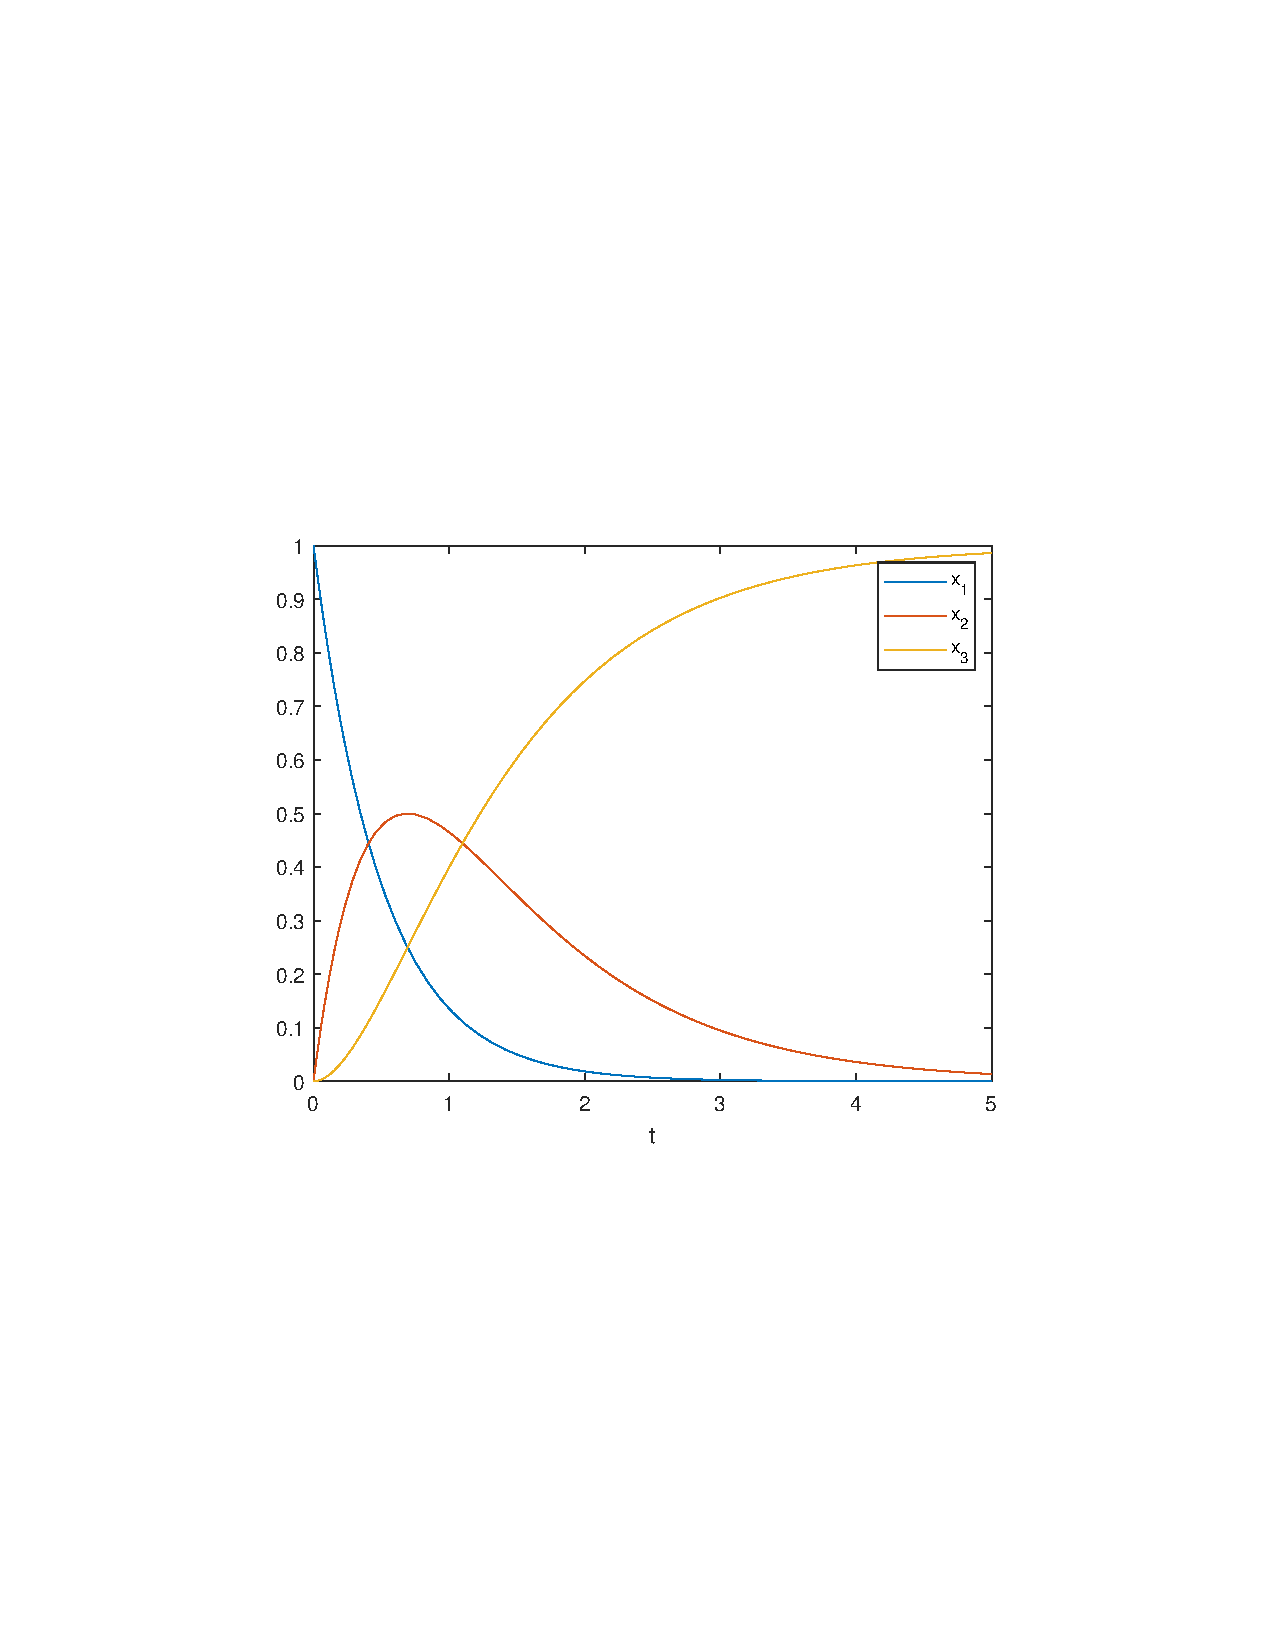
\includegraphics[width=\linewidth/2]{./code_ch1/exer1.pdf}
    \caption{system simulation}
    \label{fig:exer1-1}
\end{figure}
\end{answer}

\begin{exercise} Distributed systems and time delay.\\
We assume familiarity with the transfer function of a time delay from an undergraduate systems course
\begin{equation}
    \bar{y}(s)=e^{-\theta s}\bar{u}(s)
\end{equation}
Let's see the connection between the delay and the distributed systems, which give rise to it. A simple physical example of a time delay caused by transport in a flowing system. Consider plug flow in a tube depicted in Fig.\ref{fig:exer1-2}.

\begin{figure}[htbp]
\centering
\tikzset{every picture/.style={line width=0.75pt}} %set default line width to 0.75pt        
\begin{tikzpicture}[x=0.75pt,y=0.75pt,yscale=-1,xscale=1]
%uncomment if require: \path (0,185); %set diagram left start at 0, and has height of 185

%Shape: Ellipse [id:dp19295851654284357] 
\draw   (272,42) .. controls (283.05,42) and (292,57.67) .. (292,77) .. controls (292,96.33) and (283.05,112) .. (272,112) .. controls (260.95,112) and (252,96.33) .. (252,77) .. controls (252,57.67) and (260.95,42) .. (272,42) -- cycle ;
%Straight Lines [id:da7486939098222503] 
\draw    (272,42) -- (399.44,42) ;
%Straight Lines [id:da3129886311233703] 
\draw    (272,112) -- (399.44,112) ;
%Shape: Arc [id:dp1273018290846848] 
\draw  [draw opacity=0] (399.44,42) .. controls (399.44,42) and (399.44,42) .. (399.44,42) .. controls (399.44,42) and (399.44,42) .. (399.44,42) .. controls (410.49,42) and (419.44,57.67) .. (419.44,77) .. controls (419.44,96.33) and (410.49,112) .. (399.44,112) -- (399.44,77) -- cycle ; \draw   (399.44,42) .. controls (399.44,42) and (399.44,42) .. (399.44,42) .. controls (399.44,42) and (399.44,42) .. (399.44,42) .. controls (410.49,42) and (419.44,57.67) .. (419.44,77) .. controls (419.44,96.33) and (410.49,112) .. (399.44,112) ;  
%Straight Lines [id:da8609030882922339] 
\draw    (123,76.67) -- (237.44,77.32) ;
\draw [shift={(239.44,77.33)}, rotate = 180.33] [color={rgb, 255:red, 0; green, 0; blue, 0 }  ][line width=0.75]    (10.93,-3.29) .. controls (6.95,-1.4) and (3.31,-0.3) .. (0,0) .. controls (3.31,0.3) and (6.95,1.4) .. (10.93,3.29)   ;
%Straight Lines [id:da8626778179325296] 
\draw    (437.44,77.33) -- (536.11,77.33) ;
\draw [shift={(538.11,77.33)}, rotate = 180] [color={rgb, 255:red, 0; green, 0; blue, 0 }  ][line width=0.75]    (10.93,-3.29) .. controls (6.95,-1.4) and (3.31,-0.3) .. (0,0) .. controls (3.31,0.3) and (6.95,1.4) .. (10.93,3.29)   ;

% Text Node
\draw (124,41.4) node [anchor=north west][inner sep=0.75pt]    {$c_{j} \ ( 0,t) =u( t)$};
% Text Node
\draw (124,84.4) node [anchor=north west][inner sep=0.75pt]    {$v$};
% Text Node
\draw (252,118.4) node [anchor=north west][inner sep=0.75pt]    {$z=0$};
% Text Node
\draw (390,123.4) node [anchor=north west][inner sep=0.75pt]    {$z=L$};
% Text Node
\draw (439,41.4) node [anchor=north west][inner sep=0.75pt]    {$c_{j} \ ( 0,t) =y( t)$};
\end{tikzpicture}
\caption{Plug-flow reactor}
\label{fig:exer1-2}
\end{figure}

\begin{enumerate}[label=(\alph*)]
    \item Write down the equation of change for moles of component $j$ for an arbitrary volume element and show that
    \begin{equation}
        \pdv{c_j}{t}=-\nabla \cdot (c_j v_j)+R_j
    \end{equation}
    in which $c_j$ is the molar concentration of component $j$, $v_j$ is the velocity of component $j$, and $R_j$ is the production rate of component $j$ due to chemical reaction.

    Plug flow means the fluid velocity of all components os purely in the $z$ direction, and os independent of $r$ and $\theta$ and, we assume here, z
    \begin{equation}
        v_j=v\delta_z
    \end{equation}
    
    \item Assuming plug flow and neglecting chemical reaction in the tube, show that the equation of change reduces to 
    \begin{equation}\label{equ:exer1-2}
        \pdv{c_j}{t}=-v\pdv{c_j}{z}
    \end{equation}
    This equation is known as a hyperbolic, first-order partial differential equation.
    \begin{alignat}{3}
        &c_j(z,t)=u(t) &&0=z &&t\ge 0  \\
        &c_j(z,t)=c_{j0}(t) \quad &&0\le z\le L\quad &&t=0 
    \end{alignat}
    In other words, we are using the feed concentration as the manipulated variable, $u(t)$, and the tube starts out with some initial concentration profile of component $j$, $c_{j0}(z)$.
    
    \item Show that the solution to \eqref{equ:exer1-2} with these boundary conditions is 
    \begin{equation}
        c_j(z,t) = 
        \begin{cases}
            u(t-z/v) & \quad vt>z\\
            c_{j0}(z-vt) & \quad vt<z\\ 
        \end{cases}
    \end{equation}
    \item If the reactor start out empty of component $j$, show that the transfer function between the outlet concentration, $y=c_j(L,t)$, and the inlet concentration, $c_j(0,t)=u(t)$, is a time delay. What is the value of $\theta$?
\end{enumerate}
\end{exercise}

\begin{answer}
\begin{enumerate}[label=(\alph*)]
    \item let $f$ be the moles of one of the component, then from 3D Leibniz formula, we get 
    \begin{equation}
        \pdv{c_j}{t}=\dv{}{t}\int_{V}f(\vec x,t)~\mathrm{d}V = 
        \int_V \pdv{f}{t}~\mathrm{d}V - 
        \int_A f\vec v\cdot \vec n\mathrm~{d}V
    \end{equation}
    where $V$ is a small unit volume, $A$ is the responding surface, $v$ represent the velocity of the point on the surface, $n$ is the outward unit normal vector related to $u$.\\
    By using Gauss divergence theorem, we know that
    \begin{equation}
        \int_V \pdv{f}{t}~\mathrm{d}V -
        \int_A f\vec v\cdot \vec n~\mathrm{d}V =
        \int_V \pdv{f}{t} - \nabla \cdot f\vec v~\mathrm{d}V = 
        -\nabla\cdot(c_j v_j)+R_j
    \end{equation} 
    where the last equation comes from $v_j=v\delta_z$.

    \item Neglecting chemical reaction in the tube, we get $R_j=0$. Then we know that
    \begin{equation}
        \pdv{c_j}{t}=-\nabla\cdot(c_j v_j)=
        -\left(\pdv{}{x}\delta_x+\pdv{}{y}\delta_y+\pdv{}{z}\delta_z\right)\cdot v\delta_z=-v\pdv{c_j}{z}
    \end{equation}

    \item Assuming that $u(t-z/v)=c_{j0}(z-vt)$ when $vt<z$, we just need to prove the solution is $c_j(z,t)=u(t-z/v)$. The variables of original partial differential equation has already been separated, so we get $c_j(z,t)=u(t-z/v)$ easily from the method of characteristics.

    \item We know that $y=u(t-L/v)$, which is a time delay. The value of $\theta$ could be $L/v$.
\end{enumerate}
\end{answer}


\begin{exercise} Pendulum in the state space.\\
    Consider the pendulum suspended at the end of a rigid link depicted in Figure \ref{fig:exer1-3}. Let $r$ and $\theta$ denote the polar coordinates of the center of the pendulum, and let $p=r\delta_r$ be the position vector of the pendulum, in which $\delta_r$ and $\delta_\theta$ are the unit vectors in polar coordinates. We wish to determine a state space description of the system. We are able to apply a torque $T$ to the pendulum as our manipulated variable. The pendulum has mass $m$, the only other external force acting on the pendulum is gravity, and we neglect friction. The link provides force $-t\delta_r$ necessary to maintain the pendulum at distance $r=R$ from the axis of rotation, and we measure the force $t$.
    \begin{enumerate}[label=(\alph*)]
        \item Provide expressions for the four partial derivatives for changes in the unit vectors with $r$ and $\theta$
        \begin{equation}
            \pdv{\delta_r}{r}\quad
            \pdv{\delta_r}{\theta}\quad
            \pdv{\delta_\theta}{r}\quad
            \pdv{\delta_\theta}{\theta}
        \end{equation}
        \item Use the chain rule to find the velocity of the pendulum in terms of the time derivatives of $r$ and $\theta$. Do not simplify yet by assuming $r$ is constant. We want the general result.
        \item Differentiate again to show that the acceleration of the pendulum is
        \begin{equation}
            \ddot{p}=(\ddot{r}-r\dot{\theta}^2)\delta_r+(r\ddot{\theta}+2\dot r\dot \theta)\delta_\theta
        \end{equation}
        \item Use a momentum balance on the pendulum mass (you may assume it is a point mass) to determine both the force exerted by the link
        \begin{equation}
            t=mR\dot{\theta}^2+mg\cos \theta
        \end{equation}
        and an equation for the pendulum due to gravity and the applied torque 
        \begin{equation}
            mR\ddot \theta-T/R+mg\sin \theta=0
        \end{equation}
        \item Define a state vector and give a state space description of your system. What is the physical significance of your state. Assume you measure the force exerted by the link. 

        One answer is 
        \begin{align}
            \dv{x_1}{t}&=x_2\\
            \dv{x_2}{t}&=-(g/R)\sin x_1 + u\\
            y&=mRx_2^2+mg\cos x_1
        \end{align}
        in which $u=T/(mR)$
    \end{enumerate}

    \begin{figure}[htbp]
        \centering
        \tikzset{every picture/.style={line width=0.75pt}} %set default line width to 0.75pt        
        \begin{tikzpicture}[x=0.75pt,y=0.75pt,yscale=-1,xscale=1]
        %uncomment if require: \path (0,314); %set diagram left start at 0, and has height of 314

        %Shape: Circle [id:dp2950011826534309] 
        \draw   (292,68.56) .. controls (292,63.52) and (296.08,59.44) .. (301.11,59.44) .. controls (306.14,59.44) and (310.22,63.52) .. (310.22,68.56) .. controls (310.22,73.59) and (306.14,77.67) .. (301.11,77.67) .. controls (296.08,77.67) and (292,73.59) .. (292,68.56) -- cycle ;
        %Straight Lines [id:da090033932413494] 
        \draw    (301.11,68.56) -- (301.11,296.11) ;
        %Straight Lines [id:da4699536388586447] 
        \draw    (301.11,77.67) -- (401.11,177.67) ;
        %Straight Lines [id:da6389033949732379] 
        \draw    (310.22,68.56) -- (410.22,168.56) ;
        %Shape: Circle [id:dp07724480337773221] 
        \draw   (397.56,191.11) .. controls (397.56,177.3) and (408.75,166.11) .. (422.56,166.11) .. controls (436.36,166.11) and (447.56,177.3) .. (447.56,191.11) .. controls (447.56,204.92) and (436.36,216.11) .. (422.56,216.11) .. controls (408.75,216.11) and (397.56,204.92) .. (397.56,191.11) -- cycle ;
        %Straight Lines [id:da5473757293168724] 
        \draw    (422.56,216.11) -- (422.56,295.78) ;
        \draw [shift={(422.56,298.78)}, rotate = 270] [fill={rgb, 255:red, 0; green, 0; blue, 0 }  ][line width=0.08]  [draw opacity=0] (8.93,-4.29) -- (0,0) -- (8.93,4.29) -- cycle    ;
        %Shape: Arc [id:dp03303639601363284] 
        \draw  [draw opacity=0] (340.52,49.02) .. controls (349.47,67.04) and (345.1,89.49) .. (328.82,102.7) .. controls (309.96,118.01) and (282.27,115.12) .. (266.97,96.27) .. controls (263.64,92.16) and (261.17,87.64) .. (259.54,82.92) -- (301.11,68.56) -- cycle ; \draw   (340.52,49.02) .. controls (349.47,67.04) and (345.1,89.49) .. (328.82,102.7) .. controls (309.96,118.01) and (282.27,115.12) .. (266.97,96.27) .. controls (263.64,92.16) and (261.17,87.64) .. (259.54,82.92) ;  
        %Straight Lines [id:da5790277832441415] 
        \draw    (340.52,49.02) -- (338.83,45.2) ;
        \draw [shift={(337.62,42.45)}, rotate = 66.18] [fill={rgb, 255:red, 0; green, 0; blue, 0 }  ][line width=0.08]  [draw opacity=0] (8.93,-4.29) -- (0,0) -- (8.93,4.29) -- cycle    ;
        %Shape: Arc [id:dp13698095777819153] 
        \draw  [draw opacity=0] (369.14,146.35) .. controls (362.68,152) and (355.4,156.92) .. (347.37,160.94) .. controls (332.57,168.36) and (316.83,171.88) .. (301.33,171.9) -- (301.11,68.56) -- cycle ; \draw   (369.14,146.35) .. controls (362.68,152) and (355.4,156.92) .. (347.37,160.94) .. controls (332.57,168.36) and (316.83,171.88) .. (301.33,171.9) ;  
        %Straight Lines [id:da16810105436476697] 
        \draw    (363.08,151) -- (366.76,148.18) ;
        \draw [shift={(369.14,146.35)}, rotate = 142.52] [fill={rgb, 255:red, 0; green, 0; blue, 0 }  ][line width=0.08]  [draw opacity=0] (8.93,-4.29) -- (0,0) -- (8.93,4.29) -- cycle    ;

        % Text Node
        \draw (430.58,241.07) node [anchor=north west][inner sep=0.75pt]    {$g$};
        % Text Node
        \draw (454.92,181.07) node [anchor=north west][inner sep=0.75pt]    {$m$};
        % Text Node
        \draw (336.67,168.32) node [anchor=north west][inner sep=0.75pt]    {$\theta $};
        % Text Node
        \draw (399.25,133.82) node [anchor=north west][inner sep=0.75pt]    {$r$};
        % Text Node
        \draw (351.67,55.9) node [anchor=north west][inner sep=0.75pt]    {$T$};

        \end{tikzpicture}
        \caption{Pendulum with applied torque}
        \label{fig:exer1-3}
        \end{figure}
\end{exercise}

\begin{answer}
\begin{enumerate}[label=(\alph*)]
    \item we assume that $\delta_\theta$ is rotated from $\delta$ by anticlockwise.
    \begin{equation}
        \pdv{\delta_r}{r}=0 \quad
        \pdv{\delta_r}{\theta}=\delta_\theta \quad
        \pdv{\delta_\theta}{r}=0 \quad
        \pdv{\delta_\theta}{\theta}=-\delta_r
    \end{equation} 
    \item Since $p=r\delta_r$
    \begin{equation}
        \dot p=\dot r\delta_r+r\pdv{\delta_r}{t}
        =\dot r\delta_r+r\pdv{\delta_r}{\theta}\dot\theta
        =\dot r\delta_r+r\dot\theta\delta_\theta
    \end{equation}
    \item Differentiate again
    \begin{align}
        \ddot p&=\ddot r \delta_r+\dot r\dot\theta\delta_\theta+r\ddot\theta\delta_\theta+r\dot\theta\left(-\delta_r\dot\theta\right)+\dot r\dot\theta\delta_\theta\\
        &=\left(\ddot r-r\dot\theta^2\right)\delta_r+\left(r\ddot\theta+2\dot r\dot\theta\right)\delta_\theta
    \end{align}
    \item By the Newton's second law of motion, we get
    \begin{equation}
        F=-t\delta_r+T/R \delta_\theta+mg\sin\theta\delta_r+mg\cos\theta\delta_\theta=-mR\dot\theta^2\delta_r
    \end{equation}
    Simplify it by two direction
    \begin{align}
        &t=mR\dot\theta^2+mg\cos\theta\\
        &mR\ddot\theta-T/R+mg\sin\theta=0
    \end{align}
    \item State vector could be $x=[\theta,\dot \theta]^\top$, and the system
    \begin{align}
        \dot x&=\begin{bmatrix}
            \dot \theta\\
            \ddot \theta
        \end{bmatrix}=
        \begin{bmatrix}
            \dot \theta\\
            -g\sin\theta/R+T/\left(mR^2\right)
        \end{bmatrix}\\
        y&=\theta
    \end{align}
\end{enumerate}
\end{answer}

\begin{exercise} Time to Laplace domain.\\
Take the Laplace transform of the following set of differential equations and find the transfer function, $G(s)$, connecting $\bar u(s)$ and $\bar y(s)$, $\bar y=G\bar u$
\begin{align}\label{equ:exer1-4}
    \dv{x}{t}&=Ax+Bu\\
    y&=Cx+Du
\end{align}
For $x\in\mathbb R^n$, $y\in\mathbb R^p$, and $u\in\mathbb R^m$, what is the dimension of the $G$ matrix? What happens to the initial condition, $x(0)=x_0$? 
\end{exercise}

\begin{answer}
The Laplace transform of the differential equation is 
\begin{equation}
    sx=Ax+Bu
\end{equation}
and the transfer function
\begin{equation}
    G(s)=C(sI-A)^{-1}B\in\mathbb{R}^{p\times m}
\end{equation}
the initial condition does not appear in the Laplace transform, because the Laplace transform explains the dynamic from $u$ to $y$, and when we need to determine the accurate trajectory of the system, the initial condition is needed by inverse Laplace transform.
\end{answer}

\begin{exercise} Converting between continuous and discrete time models.\\
Given a prescribed $u(t)$, derive and check the solution to \eqref{equ:exer1-4}. Given a prescribed $u(k)$ sequence, what is the solution to the discrete time model
\begin{align}
    x(k+1)&=\tilde Ax(k)+\tilde Bu(k)\\
    y(k)&=\tilde Cx(k)+\tilde Du(k)
\end{align}
\begin{enumerate}[label=(\alph*)]
    \item Compute $\tilde A$, $\tilde B$, $\tilde C$, and $\tilde D$ so that the two solutions agree at the sample times for a zero-order hold input, i.e., $y(k)=y(t_k)$ for $u(t)=u(k), t\in (t_k,t_{k+1})$ in which $t_k=k\Delta$ for sample time $\Delta$.
    \item Is your result valid for $A$ singular? If not, how can you find $\tilde A$, $\tilde B$, $\tilde C$, and $\tilde D$ for this case?
\end{enumerate}
\end{exercise}

\begin{answer}
\begin{enumerate}[label=(\alph*)]
    \item the solution to \eqref{equ:exer1-4} is
    \begin{equation}
        x(\Delta)=e^{A\Delta}x_0+\int_0^\Delta e^{A(\Delta-\tau)}Bu(\tau)\dd x
    \end{equation}
    so the accurate discrete time model is
    \begin{equation}
        \tilde{A}=e^{A\Delta}\quad\tilde B=\int_0^\Delta e^{A(\Delta-\tau)}B\dd x
        \quad\tilde{C}=C\quad\tilde{D}=D
    \end{equation}
    \item Yes, this result can be calculate normally even if A is singular.
\end{enumerate}
\end{answer}

\begin{exercise}Continuous to discrete time conversion for nonlinear models\\
Consider the autonomous nonlinear differential equation model 
\begin{align}\label{equ:exer1-6}
    \dv{x}{t}&=f(x,u)\\
    x(0)&=x_0
\end{align} 
Given a zero-order hold on the input, let $s(t,u,x_0),0\le t\le\Delta$, be the solution to \eqref{equ:exer1-6} given initial condition $x_0$ at the time $t=0$, and constant input $u$ is applied for $t$ in the interval $0\le t\le\Delta$. Consider also the nonlinear discrete time model
\begin{equation}
    x(k+1)=F(x(k),u(k))
\end{equation}
\begin{enumerate}[label=(\alph*)]
    \item What is the relationship between $F$ and $s$ so that the solution of the discrete time model agrees at the sample times with the continuous time model with a zero-order hold?
    \item Assume $f$ is linear and apply this result to check the result of Exercise 1.5.
\end{enumerate}
\end{exercise}

\begin{answer}
\begin{enumerate}[label=(\alph*)]
    \item The relationship is 
    \begin{equation}
        F(x(k),u(k))=s(\Delta,u(k-1),x(k-1))
    \end{equation}
    \item It is obvious.
\end{enumerate}
\end{answer}

\begin{exercise}Commuting functions of a matrix.\\
Although matrix multiplication does not commute in general
\begin{equation}
    AB\neq BA
\end{equation}
multiplication of functions of the same matrix do commute. You may have used the following fact in Exercise 1.5
\begin{equation}\label{equ:exer1-7}
    A^{-1}\exp{At}=\exp{At}A^{-1}
\end{equation}
\begin{enumerate}[label=(\alph*)]
    \item Prove that \eqref{equ:exer1-7} is true assuming $A$ has distinct eigenvalues and can therefore be represented as 
    \begin{equation}
        A=Q\Lambda Q^{-1}\quad 
        \Lambda=\begin{bmatrix}
            \lambda_1 &0 &\cdots &0\\
            0 &\lambda_2 &\cdots &0\\
            \vdots &\vdots &\ddots &\vdots\\
            0 &0 &\cdots &\lambda_n\\
        \end{bmatrix}
    \end{equation}
    in which $\Lambda$ is a diagonal matrix containing the eigenvalues of $A$, and $Q$ is the matrix of eigenvectors such that
    \begin{equation}
        Aq_i=\lambda_iq_i, \quad i=1,\cdots,n
    \end{equation}
    in which $q_i$ is the $i$th column of the matrix $Q$.
    \item Prove the more general relationship
    \begin{equation}\label{equ:exer1-7-2}
        f(A)g(A)=g(A)f(A)
    \end{equation}
    in which $f$ and $g$ are any functions definable by Taylor series.
    \item Prove that \eqref{equ:exer1-7-2} is true without assuming the eigenvalues are distinct.\\
    Hint: use the Taylor series defining the functions and apply the Cayley-Hamilton theorem\cite{rawlings2017model}.
\end{enumerate}
\end{exercise}

\begin{answer}
By using Cayley-Hamilton theorem, we know the matrix functions definable by Taylor series can be written in the sum of finite power terms of matrix A\cite{CayleyHamiltonTheorem}. So all the question is answered obviously by matrix commutability of finite power terms.
\end{answer}

\begin{exercise}Finite difference formula and approximating the exponential.\\
Instead of computing the exact conversion of a continuous time to a discrete time system as in Exercise 1.5, assume instead one simply approximates the time derivative with a first-order finite difference formula
\begin{equation}
    \dv{x}{t}\approx\dfrac{x(t_{k-1})-x(t_k)}{\Delta}
\end{equation}
with  step size equal to the sample time, $\Delta$. For this approximation of the continuous time system, compute $\tilde A$ and $\tilde B$ so that the discrete time system agrees with the approximate continuous time system at the sample times. Comparing these answers to the exact solution, what approximation of $e^{A\Delta}$ results from the finite difference approximation? When is this a good approximation of $e^{A\Delta}$?
\end{exercise}

\begin{answer}
In this case, the system function can be written as 
\begin{equation}
    \dfrac{x(t_{k+1})-x(t_k)}{\Delta}=Ax(t_k)+Bu(t_k)
\end{equation} 
which could be written as
\begin{equation}
    x(t_{k+1})=(I+\Delta A)x(t_k)+\Delta Bu(t_k)
\end{equation}
So $\tilde A=I+\Delta A$, $\tilde B=\Delta B$, and $e^{A\Delta}\approx I+\Delta A$. When $\Delta$ is small, this is a good approximation.
\end{answer}

\begin{exercise}Mapping eigenvalues of continuous time systems to discrete time systems.\\
Consider the continuous time differential equation and discrete equation
\begin{align}
    \dv{x}{t}&=Ax\\
    x^+&=\tilde Ax
\end{align}
and the transformation
\begin{equation}
    \tilde A=e^{A\Delta}
\end{equation}
Consider the scalar $A$ case.
\begin{enumerate}[label=(\alph*)]
    \item What $A$ represents an integrator in continuous time? What is the corresponding $A$ value for the integrator for discrete time?
    \item What $A$ give purely oscillatory solutions? What are the corresponding $\tilde A$?
    \item For what $A$ is the solution of the ODE stable? Unstable? What are the corresponding $\tilde A$?
    \item Sketch and label these $A$ and $\tilde A$ regions in two complex-plane diagrams.
\end{enumerate}
\end{exercise}

\begin{answer}
\begin{enumerate}[label=(\alph*)]
    \item In continuous time, $A=0$, and the corresponding $\tilde A=I$.
    \item $A$ with all eigenvalues on the image axis give purely oscillatory solutions, and the corresponding $\tilde A$ has all its eigenvalues on the unit circle.
    \item $A$ with all eigenvalues on the left-half plane give the solution of the ODE stable (right-half plane give the solution of the ODE unstable), and the corresponding $\tilde A$ has its all eigenvalues in the unit circle (out of the unit circle).
    \item See Fig.\ref{fig:exer1-9}. The orange area denote the stable $A$, and the blue area denote the unstable $A$.
\end{enumerate}
\begin{figure}[htbp]
    \centering

    \tikzset{every picture/.style={line width=0.75pt}} %set default line width to 0.75pt        

    \begin{tikzpicture}[x=0.75pt,y=0.75pt,yscale=-1,xscale=1]
    %uncomment if require: \path (0,300); %set diagram left start at 0, and has height of 300
    
    %Shape: Rectangle [id:dp41972077044956557] 
    \draw  [color={rgb, 255:red, 0; green, 0; blue, 0 }  ,draw opacity=0 ][fill={rgb, 255:red, 74; green, 144; blue, 226 }  ,fill opacity=0.3 ] (137.72,95.2) -- (277.06,95.2) -- (277.06,236.53) -- (137.72,236.53) -- cycle ;
    %Shape: Circle [id:dp17807459140017246] 
    \draw  [color={rgb, 255:red, 0; green, 0; blue, 0 }  ,draw opacity=0 ][fill={rgb, 255:red, 255; green, 255; blue, 255 }  ,fill opacity=1 ] (164.67,165.86) .. controls (164.67,142.27) and (183.8,123.14) .. (207.39,123.14) .. controls (230.99,123.14) and (250.11,142.27) .. (250.11,165.86) .. controls (250.11,189.46) and (230.99,208.59) .. (207.39,208.59) .. controls (183.8,208.59) and (164.67,189.46) .. (164.67,165.86) -- cycle ;
    %Shape: Circle [id:dp3951835450590713] 
    \draw  [fill={rgb, 255:red, 245; green, 152; blue, 35 }  ,fill opacity=0.3 ] (164.67,165.86) .. controls (164.67,142.27) and (183.8,123.14) .. (207.39,123.14) .. controls (230.99,123.14) and (250.11,142.27) .. (250.11,165.86) .. controls (250.11,189.46) and (230.99,208.59) .. (207.39,208.59) .. controls (183.8,208.59) and (164.67,189.46) .. (164.67,165.86) -- cycle ;
    %Shape: Axis 2D [id:dp2649968087855814] 
    \draw  (115.28,165.86) -- (295.89,165.86)(207.39,77.94) -- (207.39,249.78) (288.89,160.86) -- (295.89,165.86) -- (288.89,170.86) (202.39,84.94) -- (207.39,77.94) -- (212.39,84.94)  ;
    %Shape: Rectangle [id:dp3122182305712575] 
    \draw  [color={rgb, 255:red, 0; green, 0; blue, 0 }  ,draw opacity=0 ][fill={rgb, 255:red, 74; green, 144; blue, 226 }  ,fill opacity=0.3 ] (442.72,95.2) -- (512.39,95.2) -- (512.39,236.53) -- (442.72,236.53) -- cycle ;
    %Shape: Axis 2D [id:dp6823514523283494] 
    \draw  (350.62,165.86) -- (531.22,165.86)(442.72,77.94) -- (442.72,249.78) (524.22,160.86) -- (531.22,165.86) -- (524.22,170.86) (437.72,84.94) -- (442.72,77.94) -- (447.72,84.94)  ;
    %Shape: Rectangle [id:dp9907477927724002] 
    \draw  [color={rgb, 255:red, 0; green, 0; blue, 0 }  ,draw opacity=0 ][fill={rgb, 255:red, 245; green, 152; blue, 35 }  ,fill opacity=0.25 ] (373.06,95.2) -- (442.72,95.2) -- (442.72,236.53) -- (373.06,236.53) -- cycle ;
    
    % Text Node
    \draw (285.33,175.33) node [anchor=north west][inner sep=0.75pt]   [align=left] {Real};
    % Text Node
    \draw (218,74) node [anchor=north west][inner sep=0.75pt]   [align=left] {Image};
    % Text Node
    \draw (190.67,167.07) node [anchor=north west][inner sep=0.75pt]    {$O$};
    % Text Node
    \draw (252.11,169.26) node [anchor=north west][inner sep=0.75pt]    {$1$};
    % Text Node
    \draw (520.67,175.33) node [anchor=north west][inner sep=0.75pt]   [align=left] {Real};
    % Text Node
    \draw (453.33,74) node [anchor=north west][inner sep=0.75pt]   [align=left] {Image};
    % Text Node
    \draw (426,167.07) node [anchor=north west][inner sep=0.75pt]    {$O$};
    
    
    \end{tikzpicture}
    
    \caption{Stable and Unstable $A$ and $\tilde A$ in two complex plane}
    \label{fig:exer1-9}
    \end{figure}
\end{answer}

\begin{exercise}State space realization\\
Define a state vector and realize the following models as the state models by hand. One should do a few by hand to understand what the Octave or MATLAB calls are doing. Answer the following questions. What is the connection between the poles of $G$ and the state space description? For what kinds of $G(s)$ does one obtain a nonzero $D$ matrix? What is the order and gain of these systems? Is there a connection between order and the numbers of inputs and outputs?
\begin{enumerate}[label=(\alph*)]
    \item $$G(s)=\dfrac{1}{2s+1}$$
    \item $$G(s)=\dfrac{1}{(2s+1)(3s+1)}$$
    \item $$G(s)=\dfrac{2s+1}{3s+1}$$
    \item $$y(k+1)=y(k)+2u(k)$$
    \item $$y(k+1)=a_1 y(k)+a_2 y(k-1)+b_1 u(k)+b_2 u(k-1)$$
\end{enumerate}
\end{exercise}

\begin{answer}
A state vector is an array of values that combine to represent the state of a system. It is usually composed of the variables describing the system's position and velocity, as well as any other variables that are necessary to describe its behavior. 

\begin{enumerate}[label=(\alph*)]
\item The state space representation for $G(s)=1/(2s+1)$ is:
\begin{equation}
    A = -1/2,\quad
    B = 1,\quad
    C = 1/2,\quad
    D = 0
\end{equation}

\item The state space representation for $G(s) = 1/(2s+1)(3s+1)= 3/(3s+1)-2/(2s+1)$ is:
\begin{equation}
    A = \begin{bmatrix}
         -1/2 & 0 \\
         0 & -1/3 \\
        \end{bmatrix},\quad
    B = \begin{bmatrix} 1 \\ 1 \end{bmatrix},\quad
    C = \begin{bmatrix} -1 & 1 \end{bmatrix},\quad
    D = 0
\end{equation}

\item The state space representation for $G(s) = (2s+1)/(3s+1)=2/3+1/3(3s+1)$ is:
\begin{equation}
    A = -1/3,\quad
    B = 1,\quad
    C = 1/9,\quad
    D = 2/3
\end{equation}

\item The state space representation for $y(k+1)=y(k)+2u(k)$ is:
\begin{equation}
    A = 1,\quad
    B = 2,\quad
    C = 1,\quad
    D = 0
\end{equation}

\item The state space representation for $y(k+1)=a_1 y(k)+a_2 y(k-1)+b_1 u(k)+b_2 u(k-1)$ is\cite{StateSpaceRepresentation}:
\begin{equation}
    A = \begin{bmatrix} 0 & 1 \\ a_1 & a_2 \end{bmatrix},\quad
    B = \begin{bmatrix} b_1 \\ b_2-a_1 b_1 \end{bmatrix},\quad
    C = \begin{bmatrix} 1 & 0 \end{bmatrix},\quad
    D = 0
    \end{equation}
\end{enumerate}

The connection between the poles of $G$ and the state space description is that the poles of $G$ are the eigenvalues of the matrix $A$.

For transfer functions that are not strictly proper, there will be a non-zero matrix D.

The dimension of input and output is not directly related to the dimension of system state. For non minimum implementations, the system dimension can be much larger than the input and output dimensions. It is also possible that the dimensions of the system are small, while the dimensions of the input and output are large.
\end{answer}

\begin{exercise}Minimal realization.\\    
\end{exercise}

\begin{answer}
In the previous question, the system state space representation was already a minimal realization.
\end{answer}


\begin{exercise}Partitioned matrix inversion lemma.\\
\end{exercise}

\begin{answer}
    These formulas can be directly verified by the definition of matrix inversion without complex transformation.
\end{answer}

\begin{exercise}Pertubation to an asymptotically stable linear system.\\
\end{exercise}
\begin{answer}
We know that $\rho(A)<1$, let $\epsilon=(1-\rho(A))/2$, there exists matrix norm $\|\cdot\|$ satisfy $\rho(A)<\|A\|+\epsilon$. This implies there exist $\lambda<1$ such that $\|A\|<\lambda$. So $\|x^+\|\leq \lambda \|x\|+\|B\|\|u\|$, and from the sum formula of proportional sequence, we could get $\|x^\infty\|\leq C\|u\|$, where $C$ is a real constant. So  $x\rightarrow 0$ as $u\rightarrow 0$.
\end{answer}

\begin{exercise}Exponential stability of a pertubed linear system.\\
\end{exercise}
\begin{answer}
Without losing generality, we assume $\|x_{k+1}\|\leq \lambda \|x_k\|+C\exp{-k}$, where $C$ is a real constant. Then we can get $\|x_{k}\|=eC\left(\lambda^k-e^{-k}\right)/(e\lambda-1)+\text{constant}\cdot\lambda^{k-1}$. Obviously, the state decrease exponentially to zero.
\end{answer}

\begin{exercise} Are we going forward or backward today?\\
\end{exercise}
\begin{answer}
\begin{enumerate}[label=(\alph*)]
    \item For simplicity, we use the same notation as forward DP.
    \begin{align}
        \bar{x}^0(w)&\\
        \tilde{y}^0(w) &= \bar{y}^0(\bar{x}^0(w))\\
        \tilde{z}^0(w) &= \bar{z}^0\bar{y}^0(\bar{x}^0(w))
    \end{align}
    \item Forward is more efficient, because it does not need to solve function inversion.
\end{enumerate}
\end{answer}

\begin{exercise}Method of Lagrange multipliers.\\
\end{exercise}
\begin{answer}
\begin{enumerate}[label=(\alph*)]
    \item We know that
    \begin{align}
        \pdv{L}{x}&=Hx+h-D^\top\lambda=0\\
        \pdv{L}{\lambda}&=d-Dx=0
    \end{align}
    which can be written as
    \begin{equation}
        \left[\begin{array}{c c}{{H}}&{{-D^{T}}}\\ {{-D}}&{{0}}\\ \end{array}\right]\left[\begin{array}{c}{{x}}\\ {{\lambda}}\\ \end{array}\right]=-\left[\begin{array}{c}{{h}}\\ {{d}}\\ \end{array}\right]
    \end{equation}
    \item It is obvious that $V=(1/2)x^\top Hx=(1/2)x^\top(D^\top\lambda-h)=(1/2)d^\top\lambda$.
\end{enumerate}
\end{answer}


\begin{exercise}Minimizing a constrained, quadratic function.\\
\end{exercise}
\begin{answer}
From previous exercise, we know that 
\begin{align}
    \pdv{L}{x}&=Hx-A^\top\lambda=0\\
    \pdv{L}{\lambda}&=b-Ax=0
\end{align}
So, $x=H^{-1}A^\top\lambda$. Then, $Ax=AH^{-1}A^\top\lambda=b$, $\lambda=(AH^{-1}A^\top)^{-1}b$, $x=H^{-1}A^\top(AH^{-1}A^\top)^{-1}b$, $V=(1/2)x^\top Hx=(1/2)b^\top(AH^{-1}A^\top)^{-1}b$.
\end{answer}


\begin{exercise}Minimizing a partitioned quadratic function.\\
\end{exercise}
\begin{answer}
The result can be obtained by directly substituting the matrix of this exercise into the previous exercise. The two forms of conversion can be performed through Woodbury matrix identity.
\end{answer}


\begin{exercise}Stabilizability and controllability canonical forms.\\
\end{exercise}
\begin{answer}
\begin{enumerate}[label=(\alph*)]
    \item The controllability matrix is composed of $A^kB$ in the form of column stacking. Notice that the matrix $A$ is partitioned upper triangular matrix, and $B$ has zero rows. So the controllability matrix has zero rows, and the system is not controllable.
    \item We know that
    \begin{equation}
        x_{1}\left(k\right)=\sum_{i=0}^{k-1}A_{11}^{k-i-1}B_1\cdot u\left(i\right)+\sum_{i=0}^{k-1}A_{12}x_{2}\left(i\right)+A_{11}^{k}x_1(0)
    \end{equation}
    Because $(A_{11},B_1)$ is controllable, $\sum_{i=0}^{k-1}A_{11}^{k-i-1}B_1\cdot u\left(i\right)$ has a full space image, the $x_{1}$ can be controlled from any initial state and target state. And $x_2(k)=A_{22}^k x_2(0)$ is not related to $u$, so $x_2$ are uncontrollable modes.
    
    \item Without losing generality, we assume the system is in the form of controllability canonical form. On the one hand, if a system is not stabilizable, because $(A_{11}, B_1)$ is controllable, we can know that $A_{22}$ is unstable. The unstable eigenvalue of $A_{22}$ implies for some $|\lambda|\geq 1$, $\text{rank}[\lambda I - A, B]<n$.

    On the other hand, if for some $|\lambda|\geq 1$, $\text{rank}[\lambda I - A, B]<n$, because $(A_{11}, B_1)$ is controllable, all the eigenvalues support $\text{rank}[\lambda I - A_{11}, B_1]=\text{dim}(x_1)$. So $\text{rank}[\lambda I - A_{22}, 0]<\text{dim}(x_2)$, the unstable eigenvalue comes from $A_{22}$, and the system is not stabilizing.
\end{enumerate}
\end{answer}


\begin{exercise}Regulator stability, stabilizable systems, and semidefinite state penalty.\\
\end{exercise}

\begin{answer}
\begin{enumerate}[label=(\alph*)]
    \item Without losing generality, we assume the system is in the form of controllability canonical form. 
    Because $(A,B)$ is stabilizable, there exists a sequence of $\text{dim}(x_1)$ inputs that transfers the $x_1$ to zero. When $k>\text{dim}(x_1)$, we repeat the strategy of $u$. Notice that the system trajectories start at every $x_1=0$ have the scaling of $\|x_2\|$. Because $\|x_2\|$ decrease exponentially, so the objective function $V(x,u)=\sum_{k=0}^\infty x_k^\top Qx_k+u^\top Ru$ is finite, which implies the optimization problem is feasible. On the other hand, the solution is unique since $R>0$ and the objective function is strict convex with $u$.
    So the solution of the LQR problem exists and is unique. This implies to that the objective function is non-increasing with time, and we have $x\to 0$, $u\to 0$ as $k\to 0$. The LQR is stabilizing.

    \item The difference is that $Q>0$ is replaced by $Q\ge 0$ and $(A,Q)$ detectable. We prove it by contradiction. Assume $x\to 0$ is false, then there exists $\epsilon$ such that for any $N$, when $k>N$, there exists $\|x_k\|>\epsilon$. We choose $N$ large enough, such that we can ignore sufficient small $u$ and unobservable states. For the observable states $x_3$, we expand the system function from time $k$ to time $k+\text{dim}(x_3) = k+m$, then $[y_k,\cdots, y_{k+m}]=[Q; QA;\cdots;QA^{m-1}]x_k$. Because $[Q; QA;\cdots;QA^{m-1}]$ is full rank, so the norm of $[y_k,\cdots, y_{k+m}]$ has a positive lower bound. Select $N$ repeatly, we can always find $\|Qx_k\|$ has a positive lower bound. This contradicts $x_k^\top Qx_k\to 0$. If $Q$ is not positive semidefinite or $(A,Q)$ is not detectable, the state may not convergent to zero.
\end{enumerate}
\end{answer}

\begin{exercise}Time-varying linear quadratic problem.\\
\end{exercise}
\begin{answer}
Following the chapters in the textbook, we get that
\begin{align*}
    \Pi(k-1)=&Q(k)+A(k)^\top\Pi(k)A(k)\\
    &-A(k)^\top\Pi(k)B(k)(B(k)^\top\Pi(k)B(k)+R(k))^{-1}B(k)^\top\Pi(k)A(k),~k=N,\cdots,1\\
    \Pi(N)=&Q(N),\\
    u_k^0(x)=&K(k)x,~k=N-1,\cdots,0\\
    K(k)=&-(B(k)^\top\Pi(k+1)B(k)+R(k))^{-1}B(k)^\top\Pi(k+1)A(k),~k=N-1,\cdots,0\\
    V_k^0(x)=&(1/2)x^\top\Pi(k)x
\end{align*}
Obviously, this problem also can be solved in closed form like the time-invariant case.
\end{answer}

\begin{exercise}Steady-state Riccati equation.\\
\end{exercise}
\begin{answer}
Whether it is stable A, unstable A, singular A, the final result is the same. The results obtained by iteration of Riccati equation and MATLAB function are completely consistent. the eigenvalues value of $A+BK$ is in the unit cycle. And the larger Q is, the closer the eigenvalues value of $A+BK$ is to the origin. 
\end{answer}


\begin{exercise}Positive definite Riccati iteration.\\
\end{exercise}

\begin{answer}
by Woodbury matrix identity, we get
\begin{align*}
    \Pi(k-1)&=Q+A^\top\Pi A-A^\top\Pi B(B^\top\Pi B+R)^{-1}B^\top\Pi A\\
    &=Q+A^\top(\Pi- B(B^\top\Pi B+R)^{-1}B^\top\Pi) A\\
    &=Q+A^\top(\Pi^{-1}+BR^{-1}B^\top)A>0
\end{align*}
\end{answer}

\begin{exercise}Existence and uniqueness of the solution to constrained least squares.\\
\end{exercise}
\begin{answer}
If this problem has a solution for every $b$ and the solution is unique, we know $\text{rank}(A)=p$. Otherwise, we can choose $b$ to let $Ax=b$ cannot have a solution. And we know
\begin{equation}
    \begin{bmatrix}
        Q\\A
    \end{bmatrix}x=
    \begin{bmatrix}
        A^\top \lambda \\b
    \end{bmatrix}
\end{equation}
If the rank of $[Q;A]$ is less than $n$, the problem has infinite solutions.
On the other hand, the rank condition of $A$ promise that the linear constraints always represent a subspace. And the rank condition of $[Q;A]$ promise there is unique solution.
\end{answer}


\begin{exercise}Rate-of-change penalty.\\
\end{exercise}
\begin{answer}
\begin{enumerate}[label=(\alph*)]
    \item The Riccati iteration is \cite{StanfordLQR}
    \begin{align}
        K(k)&=-(R+B^\top \Pi B)^{-1}(B^\top \Pi(t+1)A+M^\top)\\
        \Pi(k-1)&=Q+A^\top\Pi A-(A^\top\Pi B + M)(B^\top\Pi B+R)^{-1}(B^\top\Pi A+M^\top)
    \end{align}
    \item The new system is
    \begin{align}
        \begin{bmatrix}
            x(k+1)\\u(k)
        \end{bmatrix}=
        \begin{bmatrix}
            A &0\\
            0 &0
        \end{bmatrix}
        \begin{bmatrix}
            x(k)\\u(k-1)
        \end{bmatrix}+
        \begin{bmatrix}
            B\\I
        \end{bmatrix}u(k)
    \end{align}
    \begin{equation}
        \Delta u(k)=u(k)-[0~I]\tilde x(k)
    \end{equation}
    The new matric are
    \begin{align}
        &x^\top Qx+u^\top Ru+\Delta u^\top S \Delta u  \\
        =~&\tilde x^\top
        \begin{bmatrix}
            Q &0\\ 0 &S
        \end{bmatrix}
        \tilde x
        +u^\top (R+S)u
        -2\tilde x^\top \begin{bmatrix}0\\S\end{bmatrix} u
    \end{align}
\end{enumerate}
\end{answer}


\begin{exercise}Existence, uniqueness and stability with the cross term.\\
\end{exercise}
\begin{answer}
The reparameterizing is
\begin{equation}
    v=u+R^{-1}M^\top x
\end{equation}
and the new value function is 
\begin{equation}
    V=(1/2)\sum_{k=0}^\infty x(k)^\top(Q-MR^{-1}M^\top)+v(k)^\top R v(k)
\end{equation}
and the system changes to
\begin{equation}
    x(k+1)=(A-BR^{-1}M^\top)x(k)+Bv(k)
\end{equation}
the existence, uniqueness and stability conditions are $(A-BR^{-1}M^\top,B)$ stabilizable, $Q-MR^{-1}M^\top\ge 0$, $(A-BR^{-1}M^\top, Q-MR^{-1}M^\top)$ detectable, and $R\ge 0$.
\end{answer}

\begin{exercise}Forecasting and variance increase or decrease.\\
\end{exercise}
\begin{answer}
\begin{enumerate}[label=(\alph*)]
    \item A counterexample
    \begin{equation}
        A=
        \begin{bmatrix}
        0 & 1/2 \\
        1/2 & 0 \\
        \end{bmatrix},\quad
        P=
        \begin{bmatrix}
        1 & 0 \\
        0 & 100 \\
        \end{bmatrix}
    \end{equation}
    \item A counterexample
    \begin{equation}
        A=
        \begin{bmatrix}
        0 & 2 \\
        2 & 0 \\
        \end{bmatrix},\quad
        P=
        \begin{bmatrix}
        1 & 0 \\
        0 & 100 \\
        \end{bmatrix}
    \end{equation}
    \item A counterexample
    \begin{equation}
        A=
        \begin{bmatrix}
        0 & 2 \\
        2 & 0 \\
        \end{bmatrix},\quad
        P=
        \begin{bmatrix}
        1 & 0 \\
        0 & 100 \\
        \end{bmatrix}
    \end{equation}
\end{enumerate}
\end{answer}


\begin{exercise}Convergence of MHE with zero prior weighting.\\
\end{exercise}
\begin{answer}
In the absence of noise, if the data length is greater than the observability index, the unique solution can be obtained. When the data is insufficient, the solution belong to a linear subspace. When the data reaches the observability index, the initial state can be directly calculated, and the optimization has unique solution.
\end{answer}

\begin{exercise}Symmetry in regulation and estimation.\\
\end{exercise}
\begin{answer}
After tedious calculation, the conclusion shown in the exercise is obvious.
\end{answer}


\begin{exercise}Symmetry in the Riccati iteration.\\
\end{exercise}
\begin{answer}
    The conclusion is obvious through variable replacement.
\end{answer}


\begin{exercise}Detectability and observability canonical forms.\\
\end{exercise}
\begin{answer}
This is the dual of answer 19. Only need to transpose the matrix.
\end{answer}


\begin{exercise}Estimator stability and detectable systems.\\
\end{exercise}
\begin{answer}
From the perspective of observability canonical form, the observable state still satisfies Lemma 1.6. And it is obvious that the norm of unobservable state is controlled by the norm of observable, so the estimator is stable. (By the way, it seems that there is no definition of estimator stability.)
\end{answer}


\begin{exercise}Estimator stability and semidefinite state noise penalty.\\
\end{exercise}
\begin{answer}
\begin{enumerate}[label=(\alph*)]
    \item Because $Q$ is positive semidefinite, $Q=M^\top M,~M\in \mathbb{R}^{\text{rank}(Q)\times n}$, where $M$ has full rank. So $G=M^\top,~\tilde Q=MM^\top$.
    Perform a invertible transformation on the system so that only the first $\text{rank}(Q)$ column of $B$ is non-zero, then delete all zero columns of $B$ and delete the corresponding control input. Transform the system back and get $G\in \mathbb{R}^{n\times \text{rank}(Q)},\tilde Q=G^\top G\in \mathbb{R}^{\text{rank}(Q)\times \text{rank}(Q)}$.
    \item The noise is not independent, but linearly correlated.
    \item This is obvious from the way G is constructed in the first question.
    \item The difference between this question and Exercise 1.32 is that here $(A,G)$ is stabilizable. For uncontrollable modes, as time increases, it will converge to zero, so the error is bounded. For controllable modes, that does not satisfy the system equation cannot increase the norm of $w$, so the term w in the objective function is zero only when the system equation is satisfied, so the estimator will not be unstable.
    \item The estimator will be unstable and the state may diverge.
\end{enumerate}
\end{answer}


\begin{exercise}Calculating mean and variance form data.\\
\end{exercise}
\begin{answer}
\begin{enumerate}[label=(\alph*)]
    \item We know that 
    \begin{equation}
        \mathbb{E}\hat x=\mathbb{E}\dfrac{1}{N} \sum^N_k x_k=\dfrac{1}{N} \sum^N_k \mathbb{E}x_k=\mathbb{E}x
    \end{equation}
    \item We know that 
    \begin{align}
        \mathbb{E}\hat P
        &=\dfrac{1}{N}\mathbb{E}\sum^N_k\left(x_k-\dfrac{1}{N} \sum^N_k x_k\right)^2\\
        &=\dfrac{1}{N}\mathbb{E}\sum^N_k x_k^2
        +\mathbb{E}\sum^N_k\left(\dfrac{1}{N} \sum^N_k x_k\right)^2
        -\dfrac{2}{N}\mathbb{E}\sum^N_k\left(x_k\dfrac{1}{N} \sum^N_k x_k\right)^2\\
        &=\dfrac{N-1}{N}\mathbb{E}\sum^N_k\left(\mathbb{E}x-\dfrac{1}{N} \sum^N_k x_k\right)^2\\
        &=\dfrac{N-1}{N}P
    \end{align}
    \item the unbiased estimate is
    \begin{align}
        \hat P
        &=\dfrac{N}{N-1}\sum^N_k\left(x_k-\dfrac{1}{N} \sum^N_k x_k\right)^2
    \end{align}
    \item $N\ge 100$.
\end{enumerate}
\end{answer}


\begin{exercise}Expected sum of squares.\\
\end{exercise}
\begin{answer}
We focus on one of the quadratic summation terms
\begin{equation}
    \mathbb{E}(x_i x_j q_{ij})
    =q_{ij}\mathbb{E}(x_i x_j)
    =q_{ij}\left(\mathbb{E}(x_i)\mathbb{E}(x_j)+\text{Cov}(x_i,x_j)\right)
    =q_{ij} m_i m_j+q_{ij} p_{ij}
\end{equation}
And if we resum, we get what we want to prove.
\end{answer}


\begin{exercise}Normal distribution.\\
\end{exercise}
\begin{answer}
    We just have to prove that the standard normal distribution has zero mean and one variance, and the formula we want to prove in this case can be given by a linear transformation of the random variable. The symmetry of the function tells us that the mean is zero, and the variance is calculated by multiplying two identical integrals together and using polar transformations. It can also be calculated using parametric integrals. Obviously, the maximum point is taken at the mean, using what we learned about function monotonicity.
\end{answer}


\begin{exercise}Conditional densities are positive definite.\\
\end{exercise}
\begin{answer}
    Since the submatrices of a positive definite matrix are also positive definite, the first two terms hold. By Schur's complement, the last two terms are equivalent to $P$ positive definite.
\end{answer}


\begin{exercise}Expectation and covariance under linear transformations.
\end{exercise}
\begin{answer}
\begin{equation}
    \mathbb{E}Cx=C\mathbb{E}x=Cm_x
\end{equation}
\begin{equation}
    \text{Cov}(x)=\mathbb{EC}x x^\top C^\top -(\mathbb{E}Cx) (\mathbb{E}xC)^\top= Cm_x m_x^\top C^\top + CP_x C^\top- C m_x m_x^\top C^\top =CP_x C^\top
\end{equation}
\end{answer}


\begin{exercise}Normal distributions under linear transformations.\\    
\end{exercise}
\begin{answer}
    See Exercise 1.41.
\end{answer}

\begin{exercise}More on normals and linear transformations.\\
\end{exercise}
\begin{answer}
    First we prove that for random vector $X = \mu + BZ \in \mathbb{R}^{n}$, where $B$ is full rank. And the elements of random vector $Z$ is i.i.d., and is standard normal distribution. let $\Sigma = BB^{\top}$, then the PDF of $X$ is

    \[f(x) = \frac{1}{(2\pi)^{n/2}|\Sigma|^{1/2}}e^{- \frac{1}{2}(x - \mu)^{\top}\Sigma^{- 1}(x - \mu)}\]
    
    Because B is full rank, the inverse transformation of\(x \rightarrow \mu + Bx\ \) is \(\ x \rightarrow B^{- 1}(x - \mu)\ \), and the determinant of Jacobian is \(\ \left| B^{- 1} \right|\). By probability density transformation formula of multivariate random variable
    
    \begin{align}
        g(x) &= f\left( \left( B^{\top} \right)^{- 1}(x - \mu) \right)\| B^{- 1} \|\\
        &= f\left( \left( B^{\top} \right)^{- 1}(x - \mu) \right)|\Sigma|^{- \frac{1}{2}}\\
        &= \frac{1}{(2\pi)^{n/2}|\Sigma|^{1/2}}e^{- \frac{1}{2}(x - \mu)^{\top}\Sigma^{- 1}(x - \mu)}
    \end{align}

    
    where \(\ f(x) = (2\pi)^{- n/2}e^{- x^{\top}x}\ \) is the PDF of \(\ Z\ \). And \(X \sim N(\mu,BB^{\top})\).
    
    If A is a full rank square matrix, \(Y = AX + b = ABZ + A\mu + b \sim N(A\mu + b,ABB^{\top}A^{\top})\), its PDF
    
    \[h(x) = \frac{1}{(2\pi)^{n/2}\left| A\Sigma A^{\top} \right|^{1/2}}e^{- \frac{1}{2}(x - A\mu - b)^{\top}{(A\Sigma A^{\top})}^{- 1}(x - A\mu - b)}\]
    
    If A is a row full rank matrix of $m$ rows, Supplement \( AB \) with \( Q \) orthogonal to the row of \( AB \). And make it a full rank square matrix, Use 0 to supplement lines A and b
    
    \[\overline{AB} = \begin{pmatrix}
    AB \\
    Q \\
    \end{pmatrix} \in \mathbb{R}^{n \times n},\ \ \ \overline{b} = \begin{pmatrix}
    b \\
    0 \\
    \end{pmatrix} \in \mathbb{R}^{n},\ \ \ ABQ^{\top} = 0,\ \ \ \overline{A} = \begin{pmatrix}
    A \\
    Q \\
    \end{pmatrix} \in \mathbb{R}^{n \times n}\]
    
    the PDF of \(\ \overline{Y} = \overline{AB}Z + \overline{A}\mu + \overline{b}\ \) is
    
    \[\overline{h}(x) = \frac{1}{(2\pi)^{n/2}\left| \overline{AB}\left( \overline{AB} \right)^{\top} \right|^{1/2}}e^{- \frac{1}{2}\left( x - \overline{A}\mu - \overline{b} \right)^{\top}\left( \overline{AB}\left( \overline{AB} \right)^{\top} \right)^{- 1}\left( x - \overline{A}\mu - \overline{b} \right)}\]
    
    So the PDF of \(\ Y\ \) is
    
    \begin{align*}
    h(x) &= \int_{x_{m + 1},\cdots,x_{n}}^{}{\frac{1}{(2\pi)^{n/2}\left| \overline{AB}\left( \overline{AB} \right)^{\top} \right|^{1/2}}e^{- \frac{1}{2}\left( x - \overline{A}\mu - \overline{b} \right)^{\top}\left( \overline{AB}\left( \overline{AB} \right)^{\top} \right)^{- 1}\left( x - \overline{A}\mu - \overline{b} \right)}}dx\\
    &= \frac{1}{(2\pi)^{m/2}\left| A\Sigma A^{\top} \right|^{1/2}}e^{- \frac{1}{2}(x - A\mu - b)^{\top}{(A\Sigma A^{\top})}^{- 1}(x - A\mu - b)}
    \end{align*}
    
    This is because
    
    \[\int_{y}^{}{\frac{1}{(2\pi)^{(n - m)/2}\left| QQ^{\top} \right|^{1/2}}e^{- \frac{1}{2}y^{\top}\left( QQ^{\top} \right)^{- 1}y}}dx = 1,\ \ \ y = \left\lbrack x_{m + 1},\cdots,x_{n} \right\rbrack^{\top}\]
    
    Further, if the first m rows of A are full rank, and the last k row is 0, then its PDF
    
    \[h(x) = \frac{\delta(x_{i} = b_{i},i = m + 1,\cdots,n)}{(2\pi)^{m/2}\left| A\Sigma A^{\top} \right|^{1/2}}e^{- \frac{1}{2}(x - A\mu - b)^{\top}{(A\Sigma A^{\top})}^{- 1}(x - A\mu - b)}\]
    
    If the rank of non row full rank matrix $A$ is $m$, then there is an orthogonal matrix Q so that the first $m$ rows of $QA$ are full rank, and the last $k$ row is 0, that is, the PDF of \( Z=QY=QAX+Qb \) is:
    
    \[l(x) = \frac{\delta(x_{i} = (Qb)_{i},i = m + 1,\cdots,n)}{(2\pi)^{m/2}\left| QA\Sigma{(QA)}^{\top} \right|^{1/2}}e^{- \frac{1}{2}(x - QA\mu - Qb)^{\top}\left( QA\Sigma(QA)^{\top} \right)^{- 1}(x - QA\mu - Qb)}\]
    
    where \(\delta( \cdot )\ \) is a characteristic function. So the PDF of \( Y=Q ^ {- 1} Z \) is
    
    \[\frac{\delta({(Qx)}_{i} = (Qb)_{i},i = m + 1,\cdots,n)}{(2\pi)^{m/2}\left| QA\Sigma{(QA)}^{\top} \right|^{1/2}}e^{- \frac{1}{2}(Qx - QA\mu - Qb)^{\top}\left( QA\Sigma(QA)^{\top} \right)^{- 1}(Qx - QA\mu - Qb)}\]
    
    For a matrix with non full rank, it cannot be directly transformed because it leads to a positive semi definite covariance matrix, which is not allowed.
\end{answer}


\begin{exercise}Signal processing in the good old days -- recursive least squares.\\
\end{exercise}
\begin{answer}
    The iteration formula is 
    \begin{align}
        L&\leftarrow L+x^\top x,\quad L_0=P^{-1}+X^\top X\\
        R&\leftarrow L+x^\top y,\quad R_0=X^\top Y +P^{-1}\theta\\
        \hat\theta &\leftarrow L^{-1}R
    \end{align}
    By solving the optimization problem, this iterative method is obviously consistent with the solution with all the measurements.
\end{answer}


\begin{exercise}Least square parameter estimation and Bayesian estimation.\\
\end{exercise}
\begin{answer}
\begin{enumerate}[label=(\alph*)]
    \item $\hat\theta=(X^\top R X)^{-1}X^\top R(X\theta+e)$, so $\mathbb{E}~\hat\theta=(X^\top X)^{-1}X^\top(X\theta)=\theta$, and $\text{Cov}~\hat\theta=(X^\top X)^{-1}X^\top R X (X^\top X)^{-1}=\sigma^2 (X^\top X)^{-1}$.
    \item $p(\theta|y)=C p(y|\theta) p(\theta)$, where $p(y|\theta)$ is the PDF of $\mathcal{N}(X\theta,R)$. So this density is also normal too. The mean is $(X^\top X/\sigma^2 +\bar P^{-1})^{-1}(X^\top y/\sigma^2+\bar P^{-1}\bar\theta)$, the variance is $(X^\top X/\sigma^2 +\bar P^{-1})^{-1}$.
    \item If $\bar P^{-1}\rightarrow 0$, $m\rightarrow (X^\top X)^{-1}X^\top y$, $P\rightarrow \sigma^2 (X^\top X)^{-1}$.
    \item see (a). Different from (a), the weight of quadratic form here is $R$.
    \item see (a).
    \item $p(\theta|y)=C p(y|\theta) p(\theta)$, where $p(y|\theta)$ is the PDF of $\mathcal{N}(X\theta,R)$. So this density is also normal too. The mean is $(X^\top R X +\bar P^{-1})^{-1}(X^\top R y/\sigma^2+\bar P^{-1}\bar\theta)$, the variance is $(X^\top R X/\sigma^2 +\bar P^{-1})^{-1}$.
\end{enumerate}
\end{answer}


\begin{exercise}Least square and minimum varience estimation.\\
\end{exercise}
\begin{answer}
    
\end{answer}












% \chapter{Appendix A. Mathematical Background}
% Since the mathematical background is basic, we jump to the exercises section.
% \section{The solution of Exercises}
% \begin{exercise} Norms in $\mathbb{R}^n$\\
% Show that the following three functions are all norms in $\mathbb{R}^n$

% \begin{equation}\notag
%     \|x\|_2 
% \end{equation}

% \end{exercise}

\bibliographystyle{unsrt}
\bibliography{mybib}

\end{document}






















